% 
%  mainnumeric.tex
%  Numeric Cases without SMC
%  
%  Created by Sergei Vieira Silva on 2011-05-07.
%  Copyright 2011 Sergei Vieira. All rights reserved.
% 
\documentclass[]{elsarticle}
\RequirePackage[colorlinks,citecolor=blue,urlcolor=blue]{hyperref} 
\RequirePackage{hypernat}
\usepackage[latin1]{inputenc}     
%\usepackage[applemac]{inputenc}
\usepackage{graphicx}
\usepackage{pdfsync} 
\usepackage{amsmath}   
\usepackage{amssymb}    
\usepackage{cases}
%\usepackage{bbm}    
%\usepackage{amsthm}
%\usepackage{mathrsfs}
\usepackage[T1]{fontenc}
%\usepackage[default]{frcursive} %Esse pacote traz as fontes cursivas.
\usepackage{svn-multi}
\svnidlong
{$LastChangedBy: sergeidesk $}      
{$LastChangedRevision: 18 $} 
{$LastChangedDate: 2011-05-04 14:01:01 -0300 (Wed, 04 May 2011) $} 
{$HeadURL:$}

\newtheorem{theorem}{Theorem}
\newtheorem{assumption}{Assumption}
\newtheorem{acknowledgement}[theorem]{Acknowledgement}
%\newtheorem{algorithm}[theorem]{Algorithm}
%\newtheorem{axiom}[theorem]{Axiom}
%\newtheorem{case}[theorem]{Case}
%\newtheorem{claim}[theorem]{Claim}
\newtheorem{conclusion}[theorem]{Conclusion}
\newtheorem{condition}[theorem]{Condition}
\newtheorem{conjecture}[theorem]{Conjecture}
%\newtheorem{corollary}[theorem]{Corollary}
\newtheorem{corollary}{Corollary}
\newtheorem{criterion}[theorem]{Criterion}
\newtheorem{definition}{Definition}
\newtheorem{resumo}{Resumo}
\newtheorem{example}{Example}
\newtheorem{exercise}[theorem]{Exercise}
\newtheorem{lemma}{Lemma}
%\newtheorem{notation}[theorem]{Notation}
\newtheorem{principle}[theorem]{Principle}
\newtheorem{problem}[theorem]{Problem}
\newtheorem{proposition}{Proposition}
\newtheorem{remark}{Remark}
\newtheorem{remarkapp}{Remark} 
\newtheorem{solution}[theorem]{Solution}
\newtheorem{summary}[theorem]{Summary}
\newenvironment{proof}[1][Proof]{\textbf{#1} }{\rule{0.5em}{0.5em}}

\begin{document}
\begin{frontmatter}
	\title{Onedimensional Screening without Single-Crossing: Numerical Guided Approach.\footnote{Revision \textit{1.\svnrev}}} 

	\author[I,E]{A. Araujo} 
	%\corauth[cor]{Corresponding author.}
	\ead{aloisio@impa.br}
	\author[I]{S. Vieira}
	%\corauth[cor]{Corresponding author.}
	\ead{srgvie@gmail.com}
        \author[I]{C. Parra}
	%\corauth[cor]{Corresponding author.}
	\ead{carolina.parrama@gmail.com}

	\address[I]{Instituto Nacional de Matem�tica Pura e Aplicada, Estrada Dona Castorina 110, Rio de Janeiro, Brasil}
	\address[E]{Graduate School of Economics, Get�lio Vargas Foundation, Praia de Botafogo, 190, Rio de Janeiro, Brazil}

\begin{abstract}
In this paper we solve stylized problems in  
onedimensional screening without the single-crossing condition. With the aid of numerical optimization tools, we guess which are the relevant binding incentive compatibility constraints.
 Then we use this information to build a candidate solution that matches the numerical pattern.


\end{abstract}

\vspace{0.7cm}

\begin{keyword}
unidimensional screening, non single-crossing

\vspace{0.2cm}   

\textit{Palavras chaves:} screening unidimensional, no single-crossing.

\smallskip  
  
\textit{JEL Codes: D42, D82.}  
\end{keyword} 
\end{frontmatter}  
\date{}
\newpage


\section{Introduction}  
When the SMC is violated the local IC constraints are no longer sufficient for implementability
and additional (global) IC constraints have to be taken into account.\\
With the aid of numerical optimization tools, we guess which are the relevant binding incentive compatibility constraints.
       
 


\section{Model}
\label{sec:model}  
We use the Principal-Agent framework to analyse the monopolistic screening problem. In this model, each agent has a  quase-linear preference, $$V(q,t,\theta)=v(q,\theta)-t,$$
 were $t$ represents the monetary transfer. The type of consumer  $\theta \in \Theta$ is a random variable with a density $p$ positive and continuous. The firm is a profit-maximizing monopolist
which can produce any quality $q \in Q \subset \mathbb{R}_{+}$ incurring in a cost $C(q)$. $Q$ represents  the quality spectrum. The monopolist revenue is given by 
$$\Pi(q,t)= t-C(q).$$\\

Using the \textit{Revelation Principle} \footnote{The Revelation Principle has been enunciated in Gibbard [3]} the mopolist's problem can be stated as 
choosing the allocation rule $(q,t): \Theta \rightarrow \mathbb{R}_{+} \times \mathbb{R}$ that solves

\begin{equation}
\label{maxi}
 \underset{ \{ q(\cdot), t(\cdot) \}  }{max} \, \int_{\Theta} \Pi(q(\theta),t(\theta))p(\theta)d\theta,
\end{equation}

  subject to the \textit{Individual-Racionality} constraints

   $$v(q(\theta),\theta) - t(\theta) \geq 0 \, \, \forall \, \theta \in \Theta, $$

and the \textit{Incentive Compatibility} constraints

$$\theta \in arg \underset{\theta'\in \Theta}{max}  \{ v(q(\theta'),\theta) -t(\theta') \} \, \, \forall \, \theta \in \Theta. $$

\begin{remark}
 The 'Taxation Principle' \footnote{The principle can be found in Guesnerie [4], Hammond [5] and Rochet [10].} states that any allocation 
$(q,t)$ satisfying the Incentive Compatibility constraints can be implemented by a nonlinear tariff $T: Q = q(\Theta) \rightarrow \mathbb{R} $ where $$T(q(\theta))=t(\theta),\, \, \forall \, \theta \in \Theta.$$
\end{remark}

One of the greatest difficulties related to the monopolist's problem is how to deal with the IC
constraints. In general, the binding IC constraints may be determined only endogenously which
makes it a rather difficult task.

\begin{definition}
The single-crossing or Spence-Mirrlees condition (SMC) is the constant sign of the cross partial derivative with respect to decision and type\\

$\hspace{4cm} v_{q\theta} > 0 \, \, \, on \, \, Q \times \Theta \hspace{4cm} (CS_{+})$ \\
or \\ 

$\hspace{4cm} v_{q\theta} < 0 \, \, \, on \, \, Q \times \Theta \hspace{4cm} (CS_{-})$ \\
 
\end{definition}


We assume that the allocation rule $(q,t)$ is bounded and incentive compatible. The informational rent $V: \Theta \rightarrow \mathbb{R}_{+}$ is given by 
\begin{equation}
\label{renta}
V(\theta)= v(q(\theta),\theta)-t(\theta),
\end{equation}
and $T:q(\Theta) \rightarrow \mathbb{R}$ is the tariff resulting from the \textit{Revelation Principle}.

\begin{lemma}
 The tariff $T$ and the informational rent $V$ are Lipschitz continuous.
\end{lemma}
The Lemma 1 guarantees that $T$ and $V$ are a.e differentiable.

\begin{lemma} \hspace{2cm}
 \begin{enumerate}[(i)]
  \item If $V$ is differentiable at $\theta \in int(\Theta)$ and $q \in q(\theta)$, then
     \begin{equation}
      V'(\theta)=v_{\theta}(q,\theta).
      \end{equation}

  \item If $T$ is differentiable at $q \in q(\theta)\cap int(q(\Theta))$, then
     \begin{equation}
      T'(\theta)=v_{q}(q,\theta).
      \end{equation}
\end{enumerate}

\end{lemma}

Lemma 2 (ii) is the first order condition of the $\theta-$customer maximization problem $$\theta \in \underset{q\in Q}{max} \{ v(q,\theta) - T(q) \}.$$

\begin{remark}
With the SMC a decision is incentive compatible if and only if is monotonic. However, without the SMC we many have a nonmonotonic incentive compatible decision.
\end{remark}


\section{The Monopolist's Problem}
\label{sec:monopolist}
We assume the following conditions:

\begin{enumerate}[(i)]
\item $ \, v(q,\theta) \in C^{3},$
\item $ \, v_{qq} < 0$ and $v_{\theta}>0$ 
\item $ \, v_{q^2\theta} > 0 $ and $v_{q\theta^{2}} >0 ,$
\item $ \, C(0)=0,\,C'(q)>0$ and $C''(q)<0$ 
 
\end{enumerate}



Suppose that the alocation rule $(q,t)$ is incentive compatible and define the informational rent by $V(\theta)=v(q(\theta),\theta)-t(\theta)$. Let us now deduce the monopolist's maximization problem, using the same derivation as Mussa and Rosen. \\
From the definition of the informational rent
$V$ we can write the monetary transfer as $t(\theta)=v(q(\theta),\theta)-V(\theta)$ and then substitute it in equation (\ref{maxi}). The result is the following problem
\begin{equation}
 \underset{ \{q(\cdot)\} }{max} \int_{\Theta} \{  v(q(\theta),\theta) -C(q(\theta)) -V(\theta)\}d\theta.
\end{equation}

Using the Lemma 2 and integration by parts, we get $V(\theta)=\int_{\underline{\theta}}^{\theta} v_{\theta} (q(\theta),s) \,ds$ \footnote{By assumption (ii), V is increasing and we can set $V (\underline{\theta})= 0$, eliminating the IR constraints.} and we can rewrite the monopolist's problem as\\

$$\hspace{4cm} \underset{\{q(\cdot)\}}{max} \int_{\underline{\theta}}^{\overline{\theta}} f(q(\theta),\theta)p(\theta) d\theta, \hspace{4cm} (\Pi_{R})$$ 

were $f(q,\theta)=v(q(\theta),\theta)-C(q(\theta)) + \dfrac{P(\theta)-1}{p(\theta)} v_{\theta}(q(\theta),\theta).$\\


This problem is called the relaxed version of the mopolist's maximization problem. The Euler's equation gives the necessary
condition for an extremum of problem ($\Pi_{R}$).

\begin{equation}\label{euler}
 f_{q}(q,\theta)=0
\end{equation}

Let us denote the solution of equation (\ref{euler}) by $Q_{1}(\theta)$. If $Q_{1}(\theta)$ satisfies the constraints then it is the
solution of the monopolist's problem.\\

\begin{remark}
In many situations the solution of problem ($\Pi_{R}$) is far from being incentive compatible. We are going to derive the monopolist's optimization
problem in cases were the globals (IC) can be taken into account.
\end{remark}

%%%%%%%%%%%%%%%%%%%%%%%%%%%%%%%%%%%%%%%%%%%%%%%%%%%%%%%%%%%%%%%%%%%%%






Unlike the case with SMC, a decision function satisfying the first- and second-order conditions of the customer's maximization
problem may not be implementable.\\

Ara�jo and Moreira [1]  propose the following generalization of the (SMC):\\

(AM1) \, \, $v_{q\theta}(\xi,\theta)=0 $ defines a decreasing function $Q_{0}:\Theta \rightarrow \mathbb{R}_{+}$ such that 

\begin{equation}
\forall \, \theta \in \Theta \, \, v_{q\theta}(\xi,\theta) \geq 0 \Leftrightarrow \xi \geq Q_{0}(\theta).
\end{equation}

So the curve $Q_{0}$ divides the $(\theta,q)$ plane in two regions: $CS_{+}$, where $v_{q\theta} > 0$ and $CS_{-}$, where
$v_{q\theta} < 0$.\\


 In this case, without the Single-Crossing Condition, globals incentive compatibility constrains can be binding.\\

 Example, in the horizontal case ilustrated in Figure 1.\\



In this case, we will impose the global incentive compatibility constrains relating $\theta_{d}$ and $\theta_{2}$ customers. The same procedure used in [2] \footnote{i.e that the $\theta_{2}$-type does not envy $\theta_{d}$-type} impose:
\begin{equation}
 v(q({\theta_{2}}),\theta_{2}) - t(\theta_{2}) \geq v(q(\theta_{d}),\theta_{2}) - t(\theta_{d}).
\end{equation}
 
\begin{lemma}
 Consider an allocation rule $(q,t): \Theta \rightarrow \mathbb{R}_{+}\times \mathbb{R}$. If $(q,t)$ is incentive compatible then

\begin{equation}
 \int_{\hat{\theta}}^{\theta} \int_{q(\hat{\theta})}^{q(\tilde{\theta})} v_{q\theta} (\tilde{q},\tilde{\theta}) d\tilde{q} d\tilde{\theta} \geq 0, \, \, \, \forall \, \theta, \hat{\theta} \in \Theta
\end{equation}

\end{lemma}

Notice that

\begin{equation}
 0 \leq \int_{\theta_{d}}^{\theta_{2}} \int_{q(\theta_{d})}^{q(\tilde{\theta})} v_{q\theta} (\tilde{q},\tilde{\theta}) d\tilde{q} d\tilde{\theta} = \int_{\theta_{d}}^{\theta_{2}} \int_{q_{1}}^{q_{2}} v_{q\theta} (\tilde{q},\tilde{\theta}) d\tilde{q} d\tilde{\theta} + \int_{\theta_{d}}^{\theta_{2}} \int_{q_{2}}^{q(\tilde{\theta})} v_{q\theta} (\tilde{q},\tilde{\theta}) d\tilde{q} d\tilde{\theta}
\end{equation}

we can rewrite the integrals on the right hand side and determinate the isoperimetric condition (ISO).

\begin{equation}
 0 \leq \int_{\theta_{d}}^{\theta_{2}}  v_{\theta} (q(s),s)  ds - \int_{\theta_{d}}^{\theta_{2}}  v_{\theta} (q(\theta_{d}),s) ds \, \, \, (ISO)
\end{equation}

In the interval $[\theta_{d},\theta_{2}]$, we will optimally choose $q(\theta)$ such that the condition (ISO) is fulfilled. So we have the following isoperimetric problem

\begin{equation}
\label{pi_iso}
 \underset{ \{q(\cdot) \} }{max} \int_{\theta_{d}}^{\theta_{2}} f(q(\theta),\theta) d\theta 
\end{equation}
$$ s.t \, \, \, \, (ISO)$$

The following theorem can be founded in [2].

\begin{theorem}
\label{teo1}
The solution of (\ref{pi_iso}) is characterized by the following condition
\begin{equation}
 f_{q}(q,\theta) + \lambda v_{q\theta}(q,\theta) = 0
\end{equation}
were $\lambda$ is chosen to satisfy the condition (ISO) with equality.
\end{theorem}

\section{Numerical Optimization}
The monopolist's problem ($\Pi$) can be approximated by their discretization and be solved numerically  as a monopolist's problem with a finite number of types. We use the language AMPL and the solver Knitro 
for to obtain information about the solution to the problem with incentive compatibility constraints, more precisely, information about the global I.C that must be binding. This information together with the Theorem 1 allow us to find the optimal 
decision in several cases.
 





\section{Examples}
\label{sec:examp}
\subsection{$Q_{0}$ Horizontal}
\begin{itemize}
 \item $Q_{1}$ \bf{increasing} \normalfont


Given a parameter $a\in[0,\dfrac{\sqrt{2}}{2}]$, suppose that the types's $\theta$ are uniformly distributed in $[0,1]$ and their preferences  are given by

 $$v(q,\theta,a)= \theta(\dfrac{q^{2}}{2} - aq) + \theta + q$$

and the costs

 $$C(q,\theta,a)= -1 + 2\theta + q^{2}\theta + q(1 + a - \theta - 2a\theta).$$

Using the  Euler Equation  (\ref{euler}), the relaxed solution to the monopolist's problem is $Q_{1}(\theta)=\theta$ and the  curve $Q_{0}$ 
separating the regions $CS_{+}$ and $CS_{-}$ is given by a constant $Q_{0}(\theta)=a$, 

\newpage

\begin{center}
\begin{figure}[h!]
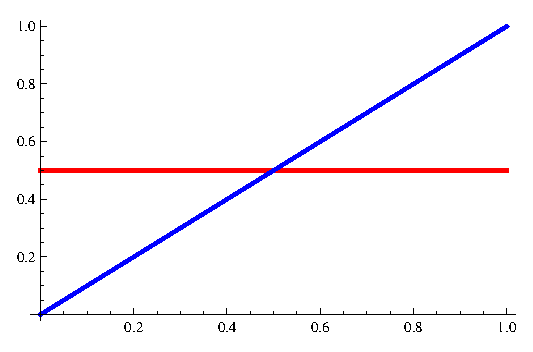
\includegraphics[scale=0.8]{hor1.eps} 
\end{figure}
Figure 1.
\end{center}

The numerical solution found by Knitro for 100 types is given by Figure 2.\\

\begin{center}
\begin{figure}[h!]
\includegraphics[scale=0.2]{knitrohor.eps} 
\end{figure}
Figure 2.
\end{center}


The numerical approach suggests that the optimal decision is a discontinuous function that consists of three parts: two flat pieces with constant decision, $q_1$ and $q_2$,
 and part of the curve relaxed $Q_{1}(\theta)$.

Thus, the optimal decision in this case, has the form $$q(\theta,a)=q_1\mathbb{I}_{[0,\theta_{d}]}(\theta,a) + q_2\mathbb{I}_{[\theta_{d}\leq \theta \leq \theta_{2}]}(\theta,a) + \theta \mathbb{I}_{[\theta_{2}\leq \theta \leq 1]}(\theta,a)$$
were $\theta_{2}=q_{2}$.\\

Monopolist's profit can be rewritten as 
\begin{equation}
 \Pi(q,\theta,a)=\int_{0}^{\theta_{d}} f(q_{1},\theta)d\theta + \int_{\theta_{d}}^{q_{2}} f(q_{2},\theta)d\theta + \int_{q_{2}}^{1} f(\theta,\theta)d\theta
\end{equation}

and the global constraint that  we consider is that the type $\theta_{2}$ does not envy $\theta_{d}$-type, which can be written, from (ISO), as
 $$\int_{\theta_{d}}^{\theta_{2}}  v_{\theta} (q_{2},s,a)  ds - \int_{\theta_{d}}^{\theta_{2}}  v_{\theta} (q(\theta_{d}),s,a) ds \geq 0$$
or, in this case
\begin{equation}
\label{iso_hor}
\int_{\theta_{d}}^{\theta_{2}}  v_{\theta} (q_{2},s,a)  ds - \int_{\theta_{d}}^{\theta_{2}}  v_{\theta} (q_{1},s,a) ds = 0
\end{equation}


\begin{center}
\begin{figure}[h!]
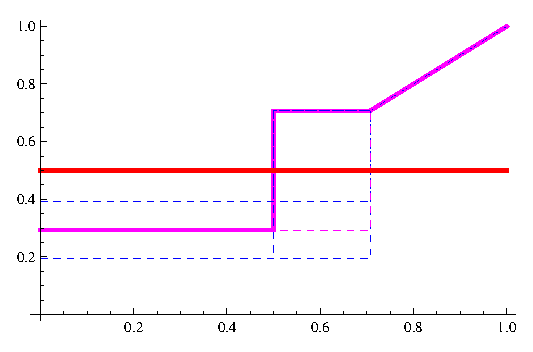
\includegraphics[scale=0.8]{iso_hor.eps} 
\end{figure}
Figure 3.
\end{center}



The equation (\ref{iso_hor}) implies the relationship $$q_{1}=2a-q_{2},$$

moreover, the continuity of $f(q,\theta,a)$ implies the additional condition 

$$f(q_{1},\theta_{d},a)=f(q_{2},\theta_{d},a)$$
 
which can be rewritten, using (ISO), as

\begin{equation}
\label{cont_hor}
 f(2a-q_{2},\theta_{d},a)-f(q_{2},\theta_{d},a)=0
\end{equation}

obtaining from (\ref{cont_hor}) the value for $\theta_{d}$,

$$\theta_{d}=a.$$

Finally, write the profit considering the global constraint (\ref{iso_hor}) as 
\begin{equation}
\label{lucro_hor}
\Pi(q_{2},a)=\int_{0}^{a} f(2a-q_{2},\theta,a) d\theta+ \int_{a}^{q_{2}} f(q_{2},\theta,a) d\theta+ \int_{q_{2}}^{1} f(\theta,\theta,a) d\theta
\end{equation}

In this (horizontal) case, the monopolist's problem without single-crossing was reduced to maximization problem with a single variable

\begin{equation}
\label{lucro_hor2}
 \underset{ \{q_{2}\} } { max } \, \Pi(q_{2},a)
\end{equation}
$$s.t \,\,\, a \leq q_{2}\leq 1$$

where the constraint $0 \leq \theta_{d} \leq \theta_{2} \leq 1$  was rewritten as   $a\leq q_{2}\leq 1$.\\

The expected profit $\Pi(q_{2},a)=\frac{1}{6}(1 - 6 a^3 + 6 a^2 q_{2} - q_{2}^3)$ is a strongly concave function in $q_{2}$ for all $a$, then the KKT optimality conditions are necessary and sufficient.\\

 Solving the problem  (\ref{lucro_hor2}) as a \textit{KKT system} we obtain the optimum values for $q_{1}$ and $q_{2}$ 

$$q_{1}(a)= 2a - \sqrt{2} a $$
$$q_{2}(a)= \sqrt{2} a.$$

So, the optimal decision is given by 
$$q(\theta,a)=(2a-\sqrt{2}a)\mathbb{I}_{[0\leq \theta \leq a ]} + \sqrt{2}a\mathbb{I}_{[a\leq \theta \leq \sqrt{2}a]}+\theta\mathbb{I}_{[\sqrt{2}a \leq \theta \leq 1]}$$


\begin{center}
\begin{figure}[h!]
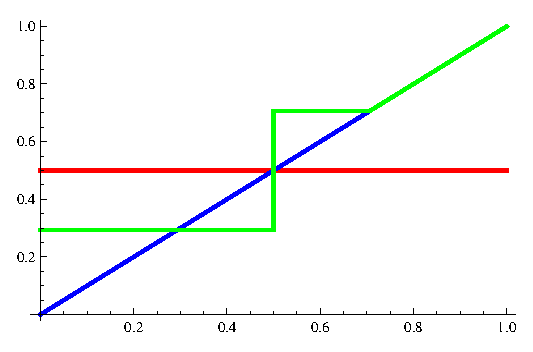
\includegraphics[scale=0.8]{completo.eps} 
\end{figure}
Figure 4.
\end{center}

\begin{center}
\begin{figure}[h!]
\includegraphics[scale=0.2]{knitroplus.eps} 
\end{figure}
Figure 5.
\end{center}




and the monopolist's expected profit from $q(\theta,a)$ is 

$$\Pi(q_{2}(a),a)=\dfrac{1}{6} (1 - 6 a^{3} + 4 \sqrt{2} a^{3})$$


%%%%%%%%% caso simetrico%%%%%%%%%%%%%%
 \vspace{1cm}

Given a parameter $a\in[\frac{3}{10},\frac{1}{2}]$, consider the types's $\theta$ uniformly distributed in $[0,1]$ with preferences given by

 $$v(q,\theta,a)= \theta(-\dfrac{q^{2}}{2} + aq) + \theta + q$$

if costs are

 $$C(q,\theta,a)= -1 - q^{2} (-1 + \theta) + 2 \theta + q (1 - \theta + a (-1 + 2 \theta)),$$


then, we get the same curves $Q_{0}$ and $Q_{1}$, but the region under the curve $Q_{0}$ is $CS_{+}$. So, we expect a decision function flat for the higher types.\\

The numerical solution found by Knitro for 100 types is given by Figure 6.\\

\begin{center}
\begin{figure}[h!]
\includegraphics[scale=0.2]{100tiposq0hor.eps} 
\end{figure}
Figure 6.
\end{center}

The numerical approach suggests that the optimal decision is a discontinuous function that consists of three parts: a first part, for the lower types, were the optimal decision is the relaxed curve $Q_{1}(\theta)$ and other two flat pieces with constant decision, $q_{1}$ and $q_{2}$, for the higher types.\\

Thus, the optimal decision in this case, has the form $$q(\theta,a)= \theta \mathbb{I}_{[0 \leq \theta \leq \theta_{1}]}(\theta,a)+ q_1\mathbb{I}_{[\theta_{1},\theta_{d}]}(\theta,a) + q_2\mathbb{I}_{[\theta_{d}\leq \theta \leq \theta_{1}]}(\theta,a) $$
were $\theta_{1}=q_{1}$.\\

Monopolist's profit can be rewritten as 
\begin{equation}
 \Pi(q,\theta,a)=\int_{0}^{q_{1}} f(\theta,\theta)d\theta + \int_{q_{1}}^{\theta_{d}} f(q_{1},\theta)d\theta + \int_{\theta_{d}}^{1} f(q_{2},\theta)d\theta
\end{equation}

From the global constraint(ISO) applied to the types $\theta_{1}$ and $\theta_{d}$ and continuity of $f$, we get the following relationships

 $$q_{1}=2a-q_{2}$$
and
$$\theta_{d}=a.$$

The monopolist's profit can be expressed as function of one  variable  


$$\Pi(q_{2},a)=\int_{0}^{2a-q_{2}} f(\theta,\theta,a) d\theta+ \int_{2a-q_{2}}^{a} f(2a-q_{2},\theta,a) d\theta+ \int_{a}^{1} f(q_2,\theta,a) d\theta$$

or

$$\Pi(q_{2},a)= \dfrac{1}{6} (2a^{3} - 6a^{2}q_{2} + 6 aq_{2}^{2} - q_{2}(-3 + 3q_{2} + q_{2}^{2})),$$

the expected profit  is a strongly concave function in $q_{2}$ for all $a\in [0, 1/2]$, then the KKT optimality conditions are necessary and sufficient.\\


Solving the problem  as a \textit{KKT system} we obtain the optimum values for $q_{1}$ and $q_{2}$ 

$$q_{1}(a)= 1 - \sqrt{2} \sqrt{(-1 + a)^2} $$
$$q_{2}(a)= -1 + \sqrt{2} \sqrt{(-1 + a)^2} + 2 a.$$

So, the optimal decision is given by 
$$q(\theta,a)=\theta \mathbb{I}_{[0\leq \theta \leq q_{1}(a) ]} + q_{1}(a)\mathbb{I}_{[q_{1}(a) \leq \theta \leq a}+ q_{2}(a) \mathbb{I}_{[a \leq \theta \leq 1]}$$


and the monopolist's expected profit from $q(\theta,a)$ is 

$$\Pi(a)=\dfrac{1}{6} (-5 + 4 \sqrt{2} \sqrt{(-1 + a)^2} + 
   2 (9 - 4 \sqrt{2} \sqrt{(-1 + a)^2}) a + 
   2 (-9 + 2 \sqrt{2} \sqrt{(-1 + a)^2}) a^2 + 6 a^3)$$

\begin{center}
\begin{figure}[h!]
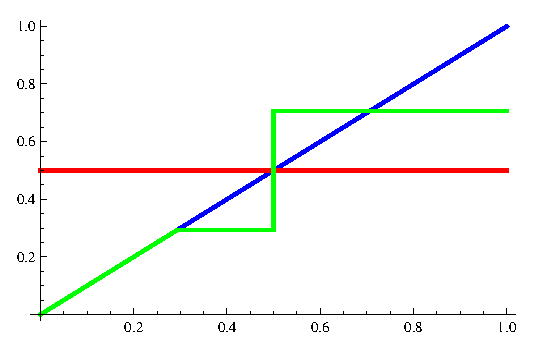
\includegraphics[scale=0.8]{hor_inv_fin.eps} 
\end{figure}
Figure 7.
\end{center}


%%%Disenhos%%%%

\item $Q_{1}$ \bf{decreasing} \\

\normalfont
With the following specifications for the distribution of types, preferences and costs  we get the same curve $Q_{0}=a$ and the relaxed solution $Q_{1}= 1 -\theta$.
 $$v(q,\theta,a)= q + \theta + (-a q + \dfrac{q^2}{2}) \theta$$


 $$C(q,\theta,a)=-1 + q^2 (-1 + \theta) + 2 \theta + q (2 + a - \theta - 2 a \theta)$$

Using the same technique as in the previous case  ((ISO) and continuity of $f$), the problem of monopoly was reduced to a one-dimensional optimization problem.\\ In the figures 8 and 9, we show the optimal decision by Knitro for the cases with $CS_{+}$ above and
 with $CS_{+}$ below, respectively. 

\begin{center}
\begin{figure}[h!]
\includegraphics[scale=0.2]{q1dec.eps} 
\end{figure}
Figure 8.
\end{center}

\newpage

\begin{center}
\begin{figure}[h!]
\includegraphics[scale=0.2]{hor_q1dec_inv.eps} 
\end{figure}
Figure 9.
\end{center}
\end{itemize}

\newpage

\subsection{$Q_{0}$ Decreasing}

Given a parameter $a\in[0,\frac{1}{3}]$, suppose that the types's $\theta$ are uniformly distributed in $[0,1]$ and their preferences  are given by

 $$v(q,\theta,a)= -(1 + a) q \theta + \frac{q^2 \theta}{2} + \frac{q \theta^{2}}{2} + q + \theta + 1,$$

and the costs

 $$C(q,\theta,a)= 2 \theta + q^2 \theta + q (1 + a - 2 \theta - 2 a \theta + \frac{3 \theta^{2}}{2}).$$

Using the  Euler Equation  (\ref{euler}), the relaxed solution and the curve $Q_{0}$ are  $Q_{1}(\theta)=1 - \theta$ 
 and $Q_{0}(\theta)=1 + a - \theta$ respectively. \\


\begin{center}
\begin{figure}[h!]
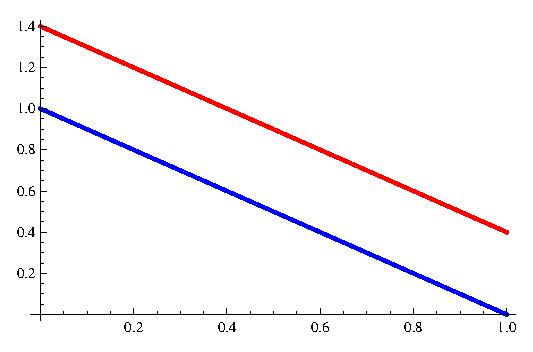
\includegraphics[scale=0.8]{q0dec.eps} 
\end{figure}
Figure 10.
\end{center}

The numerical solution found by Knitro for 100 types is given by Figure 11.\\


\begin{center}
\begin{figure}[h!]
\includegraphics[scale=0.25]{decrec.eps} 
\end{figure}
Figure 11.
\end{center}

%
\section{Conclusion}
\label{sec:conclusion}
  
 
\newpage 
%\appendix
%\input{appendix.tex}

\newpage 
%\bibliographystyle{siam}
%\bibliography{mainnumeric}

\begin{thebibliography}{11}
 \bibitem{Araujo} A. Ara\'ujo, H. Moreira, \emph{Adverse Selection Problems
without the Spence-Mirrlees Condition}. Journal of Economic Theory (Print), v. 145, p. 1113-1141, 2010.

\bibitem{Araujo} A. Ara\'ujo, H. Moreira, S. Vieira \emph{Nonlinear Pricing Beyond the Demand Profile Approach }.

\bibitem{Gibbard} A. Gibbard \emph{Manipulation for voting schemes}. Econometrica, v. 41, p. 587-601, 1973

\bibitem{Guesnerie} R. Guesnerie \emph{On taxation and incentives: further reflections on the limit of redistribution}. Mimeo, 1981.

\bibitem{Hammond} P. Hammond \emph{Straightforward individual incentive compatibility in large economies}. The Review of Economic Studies, v. 46, p. 263-282, 1979..

\bibitem{Jullien} B. Jullien \emph{Participation constraints in adverse selection models }.Journal of Economic Theory, v. 93, p. 1-47, 2000.

\bibitem{Laffont} J. J. Laffont, E. Maskin, J. C. Rochet \emph{Optimal nonlinear pricing with two dimensional characteristics }.Information, Incentives, and Economic Mechanisms: Essays in Honor of Leonid Hurwicz by Theodore Groves, Roy Radner, and Stanley Reiter, 1987.

\bibitem{Maskin} E. Maskin, J. Riley \emph{Monopoly with incomplete information}. RAND Journal of Economics, v. 15, p. 171-196, 1984.

\bibitem{Milgrom} P. Milgrom, I. Segal \emph{Envelope theorems for arbitrary choice sets}. Econometrica, v. 70, p. 583-601, 2002.

\bibitem{Rochet} J. C. Rochet \emph{A necessary and sufficient condition for rationalizability in a quasi-linear context}. Journal of Mathematical Economics, v.16, p.191-200, 1987.

\bibitem{Wilson} R.B. Wilson  \emph{Nonlinear Pricing}. Oxford University Press, 1993.

\end{thebibliography}

\end{document}

